\section{Model and methods}
\label{sec:model}
%==========================================================================

\emph{This section fixes the model, the parametrisation and the numerical conventions every
result below depends on. One model is used throughout, at three levels of detail; the
derivations, the alternative hypotheses that were rejected and the checks behind each step
are in the supplement, \S S1, and Section~\ref{sec:discussion} says what one model at three
levels of detail does and does not license.}

\subsection{Notation}

\begin{adjustwidth}{-1.0cm}{-1.0cm}
\begin{table}[htbp]
\centering
\footnotesize
\caption{\label{tab:notation}Notation, once, in one place. Values and sources are in
Table~\ref{tab:params}.}
\begin{tabular}{@{}ll@{\hskip 2em}ll@{}}
\toprule
$m$ & the plasma marker, 3-HP & $\bar m$ & the operating point, and the sample mean \\
$L(t)$ & recorded propiogenic load & $L_0$ & its \emph{unrecorded} component, unknown \\
$\theta$ & residual capacity, absorbing $V_{\max}$ & $\Delta(t)$ & therapeutic increment,
scheduled \\
$K_m$ & half-saturation, at the plasma level & $u_c(t)$ & recorded carnitine dose \\
$k_e$ & alternative clearance & $\kappa$ & its gain onto $k_e$, never assigned \\
$g(m)$ & $m/(K_m+m)$, the saturation & $\alpha(m)$ & the alternative channel, general \\
$C(m)$ & total clearance & $(a,b)$ & its affine fit over the band \\
$\Delta$ & \textbf{full} width of the band & $r$ & its fold range, $m_{\max}/m_{\min}$ \\
$\varphi(m)$ & $K_m/(K_m+m) = 1-g(m)$ & $E$ & the excitation, $\varphi$'s drop across a
band \\
$\thc$ & critical capacity & $\mu$ & the margin $\theta - \thc$, whose \emph{sign} decides \\
$\mtol$ & tolerable level, a convention & $\spk$ & illness amplitude, as a fold of baseline \\
\bottomrule
\end{tabular}
\end{table}
\end{adjustwidth}


\subsection{The dynamic model}
\label{sec:parent}

The metabolite the clinic measures is written $m$. Its balance is
\begin{equation}
\dot m \;=\; L(t) + L_0 \;-\; \bigl(\theta + \Delta(t)\bigr) g(m) \;-\; \alpha(m),
\qquad g(m) = \frac{m}{K_m + m},
\label{eq:parent}
\end{equation}
with $L$ the \emph{recorded} component of the propiogenic load, $L_0$ its unrecorded
component carried as an unknown constant, $\Delta$ the therapeutic increment known from
the dosing record, and $\alpha$ an alternative clearance route: in propionic acidemia,
principally conjugation to carnitine and renal loss of the conjugate. Carrying $L_0$ as an
unknown rather than assuming it away is what makes the identification problem well posed
at all.

The parametrisation is pinned: $\theta$ \emph{absorbs} the maximal velocity, so it
\emph{is} the patient's residual $V_{\max}$ rather than a fraction of a population one.
Carrying the two separately as $V_{\max}\theta\,g(m)$ adds a parameter no excursion
separates, since only the product multiplies $g$; splitting them needs an anchor outside
the marker, and a $1$-$^{13}$C-propionate breath test is what such an anchor looks
like~\cite{breath_test_mma}. % C48

\paragraph{Why $\alpha$ is not a rate constant.} Elimination proceeds by conjugating
propionate with carnitine, one molecule of carnitine per molecule eliminated, excreted
with the product; in two patients with propionic acidemia and two with methylmalonic
aciduria, urinary free carnitine was decreased while short-chain acylcarnitines, mostly
propionylcarnitine, were increased~\cite{carnitine_excretion_pa}. % C41
Stoichiometric consumption alone would give a ceiling rather than a decline: promote
carnitine to a state $c$ with constant replenishment, and if conjugation is its only exit
then $\dot c = 0$ fixes the conjugation flux at every $m$. What is missing is a reason for
the flux to vanish as the metabolite does and a reason for it to decline, and one mechanism
supplies both. Carnitine is recovered from the glomerular filtrate by a renal transporter
that acylcarnitines share, and in a transporter solubilised from renal apical brush-border
membrane and reconstituted into liposomes the most effective inhibitors were
acylcarnitines~\cite{octn2_renal_transport}. % C42
Propionylcarnitine rises with the metabolite, so the fraction of filtered carnitine
recovered falls as the metabolite accumulates: the free pool has a second exit, and that
exit grows with $m$. Writing $c(t)$ for available carnitine,
\begin{equation}
\begin{aligned}
\dot m &= s(t) \;-\; \theta\, g(m) \;-\; k\, c\, \frac{m}{K_c + m}, \\[2pt]
\dot c &= R_0 \;-\; k\, c\, \frac{m}{K_c + m} \;-\; \delta(m)\, c,
\qquad \delta(m) = \delta_0\left(1 + \frac{m}{M_i}\right),
\end{aligned}
\label{eq:twostate}
\end{equation}
with $K_c$ the half-saturation of the conjugation step, $\delta_0$ the basal rate of
non-conjugative loss, $M_i$ the metabolite level at which competition doubles it, and $R_0$
constant. The conjugation term is the one the two equations share, entering both with the
same coefficient, which is the one-to-one stoichiometry; they are otherwise not symmetric,
because carnitine has a second exit that propionate does not. The supplement, \S S1, draws
the system as a block diagram and works through the positive feedback it creates.

\subsection{The equilibrium reduction}
\label{sec:reduction}

\textbf{The carnitine state is not fast relative to the metabolite, and no separation of
timescales is needed to justify eliminating it.} The comparison that would be needed is
carnitine against the \emph{marker}, and it runs the wrong way: at the model's own $k$ the
carnitine time constant is $0.92$~d against the marker's $0.81$~h, slower by a factor of
$27$, and published human kinetics put whole-body carnitine turnover at $38$ to $119$~h
with a rapidly equilibrating compartment at $2$ to $3$~h (Rebouche, \emph{Ann.\ N.\ Y.\
Acad.\ Sci.} 2004), slower on either reading.

What justifies the reduction is algebraic and needs no separation at all. $\alpha$ is
\emph{defined} by solving $\dot c = 0$, and $\dot c = 0$ holds exactly at any fixed point,
so at equilibrium the two formulations are one equation rearranged, whatever the timescales
do, and everything this paper computes from the parent is computed at equilibrium. Solving
$\dot c = 0$ in \eqref{eq:twostate} for $c$ and substituting gives that flux in closed form,
\begin{equation}
\alpha(m) \;=\; R_0\,\frac{u(m)}{u(m) + \rho(m)},
\qquad u(m) = \frac{m}{K_c+m},
\qquad \rho(m) = \rho_0\left(1 + \frac{m}{M_i}\right),
\label{eq:alphaqss}
\end{equation}
with $\rho_0 = \delta_0/k$. The conjugation rate constant $k$ enters only through that
ratio and cancels from the reduced clearance, exactly. \textbf{It does not follow that $k$
is a free scale}: $k$ alone sets the carnitine relaxation rate,
$\tau_c = 1/(k[u(m) + \rho(m)])$, so it sets the reduction's validity \emph{off}
equilibrium even though it cancels from the curve, and what assuming it costs is bounded in
the $k$ row of the full registry, supplement \S S2, rather than argued away.

Setting $\dot m = 0$ gives the equilibrium reduction, which is what a steady-state fit to a
clinical record actually estimates. Its solutions are an attractor and a separatrix, and the
fold at which the two collide defines the critical capacity $\thc$: below it a sufficiently
large load leaves the system with no equilibrium at all, which is what a decompensation is
in this model. \textbf{Integrating \eqref{eq:twostate} and watching it settle on the
reduced attractor to fourteen digits is not evidence for the reduction}: it is the identity
above, so it cannot fail at any parameter value and reports nothing about the premise. The
divergence from above the separatrix needs a qualification too. Started \emph{on} the slow
manifold a trajectory a tenth of a per cent above the separatrix does run away, but started
off it, with carnitine at its pre-perturbation value, the same trajectory can return to the
attractor, so the reduced separatrix is a lower bound on the true basin and not the basin.
The intrinsic definition of $\thc$, the fold, and the comparison against the alternative
hypothesis with a ceiling instead of a fold are in the supplement, \S S1.

\subsection{The local identification model}
\label{sec:localmodel}

Linearising $\alpha \to k_e m$ gives the \emph{local identification model}, which is the one
every design calculation below uses:
\begin{equation}
\dot m \;=\; L(t) + L_0 \;-\; \bigl(\theta + \Delta(t)\bigr) g(m) \;-\; k_e\, m.
\label{eq:local}
\end{equation}

\begin{figure}[htbp]
\centering
\resizebox{0.90\linewidth}{!}{%
\begin{tikzpicture}
\node[mpool] (m) at (0,0) {$m$\\[1pt]\scriptsize\mdseries accumulated\\metabolite};
\node[mlabel] (in) at (-3.6,0) {$s(t)$};
\draw[mar] (in) -- (m);
\node[msmall] at (-2.4,0.42) {load};

\node[menzy] (enz) at (-2.3,-2.7) {$\theta\, g(m)$\\{\scriptsize saturating}};
\channelglyph{(-3.55,-4.15)}{green!45!black}{s}

\node[malt] (alt) at (2.3,-2.7) {$k_e\, m$\\{\scriptsize linear}};
\channelglyph{(1.15,-4.15)}{blue!55!black}{l}

\draw[mar] (m.south) -- ++(0,-0.55) -| (enz.north);
\draw[mar] (m.south) -- ++(0,-0.55) -| (alt.north);

\node[msmall] (o1) at (-2.3,-5.0) {eliminated};
\node[msmall] (o2) at (2.3,-5.0) {eliminated};
\draw[mar] (enz) -- (o1);
\draw[mar] (alt) -- (o2);

\node[mlabel, green!45!black] (thr) at (-6.6,-2.7) {therapy\\$\Delta(t)$};
\draw[mar, green!45!black] (thr) -- (enz);
\node[mlabel, blue!55!black] (carn) at (6.6,-2.7) {carnitine\\$u_c(t)$};
\draw[mar, blue!55!black] (carn) -- (alt);
\end{tikzpicture}}
\caption{The local identification model \eqref{eq:local} as a block diagram. One pool $m$,
filled by the load $s(t)$ and drained by two channels. The enzymatic channel saturates at
$\theta$; the alternative channel is linear in $m$, and in the \emph{unforced} model that
difference in shape is the only thing separating them. A known input that varies and rides
on one channel alone is a second and independent separator. The two selective inputs are
drawn together because, \emph{at fixed} $K_m$, they are interchangeable: carnitine acts on
$k_e$ and is recorded for every patient, the therapy acts on $\theta$ and is administered on
the published biweekly schedule, and at fixed $K_m$ the identification problem cannot tell
which one moved the patient. With $K_m$ free they are not interchangeable (supplement, \S S1); the design of Section~\ref{sec:designsec} uses the therapy.}
\label{fig:blockA}
\end{figure}


\begin{figure}[htbp]
\centering
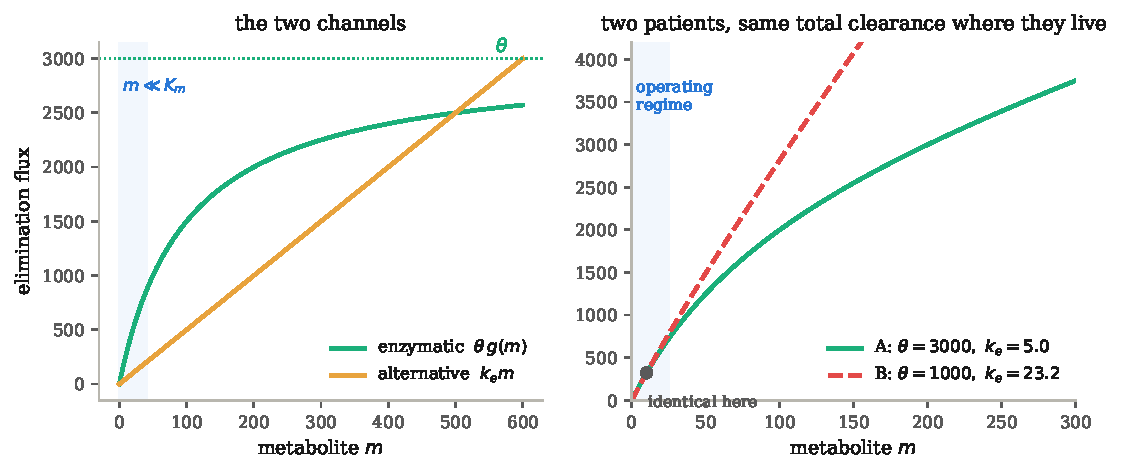
\includegraphics[width=\textwidth]{fig_A1_channels.pdf}
\caption{Left: the two elimination channels. The enzymatic term saturates at $\theta$ while
the alternative term does not, and this difference in functional form is the only thing
distinguishing them in the unforced model. In the shaded band, where clinically stable
patients are maintained, both are approximately linear, which is the difficulty the rest of
this paper is about. Right: two patients agreeing in \emph{both} the value and the slope of
total clearance at the operating point, differing only at second order. They differ
threefold in enzymatic capacity and carry different $K_m$, and no affine fit over a band
around that point tells them apart.}
\label{fig:A1}
\end{figure}


\paragraph{Why the local model is used.} It is not a reduction of the parent. The tangent
to the parent's clearance curve carries an extra term in its intercept, and at the
illustrative constants that term is $374$ against the enzymatic term's $61$, so the
alternative channel owns six-sevenths of an intercept the residual capacity was supposed to
carry. The local model is therefore a different hypothesis about one term, kept because it
is the most favourable case for identification rather than because it approximates
anything, and that is what the conclusion needs: the degeneracy this paper is about appears
in the favourable structure and disappears in the awkward one, so it is not an artefact of a
bad approximation. At matched parameter count the parent carries a degenerate family of the
same dimension, admissible over a sixteen-fold range in $K_m$ and if anything harder to
reject. What closes such a family, in either model, is an independent channel being known,
not curvature in $\alpha$. The reduction hierarchy is verified symbolically and numerically
(supplement, \S S2).

\subsection{Assumptions and their status}
\label{sec:assumed}

\begin{adjustwidth}{-1.0cm}{-1.0cm}
\scriptsize
\def\paramslabel{tab:params}
\def\paramscaption{The constants this paper reasons about, and what each rests on. Three
are from the literature and the rest are chosen for illustration, against what the last
column says. Each row also carries what \emph{kind} of quantity it is, which is a
different question from where it came from, and the species its evidence comes from where
there is one. \textbf{Some conclusions do depend on values in this table}, and the three
that decide a result are priced in the text below. The full registry is \S S2 of the
supplement, which is the authority; this is a selection from it.}
\begin{longtable}{@{}p{0.075\linewidth} p{0.085\linewidth} p{0.22\linewidth} p{0.11\linewidth} p{0.31\linewidth}@{}}
\caption{\paramscaption}\label{\paramslabel}\\
\toprule
\textbf{Symbol} & \textbf{Value} & \textbf{Meaning} & \textbf{Source} & \textbf{What the value rests on} \\
\midrule
\endfirsthead
\multicolumn{5}{@{}l}{\emph{Table \thetable, continued from the previous page}}\\
\toprule
\textbf{Symbol} & \textbf{Value} & \textbf{Meaning} & \textbf{Source} & \textbf{What the value rests on} \\
\midrule
\endhead
\midrule
\multicolumn{5}{r@{}}{\emph{continued on the next page}}\\
\endfoot
\bottomrule
\endlastfoot
\multicolumn{5}{@{}l}{\emph{The local identification model}} \\
\addlinespace[2pt]
$\bar m$ & $10$~$\mu$M & operating point: the level management holds the patient at & \textsc{assumed}\newline \emph{convention}\newline \emph{mouse} & chosen for illustration, and every design quantity is relative to it. The scale is murine~\cite{pkpd_translational}, within $1.6$ of the human newborn cut-off~\cite{dbs_3hp_cutoff} \\
$\theta$ & $3000$~$\mu$M/d & capacity of the enzymatic channel, \textbf{at normal capacity} & \textsc{assumed}\newline \emph{convention} & chosen for illustration as \emph{normal} capacity on the parent model's scale, against residual activity under $5\%$~\cite{pcc_residual_activity} \\
$\theta_{\mathrm{PA}}$ & $\le 150$~$\mu$M/d & capacity in the disease, on the scale of the row above & \textsc{literature}\newline \emph{derived}\newline \emph{human} & residual PCC activity in propionic acidemia is under $5\%$ of control~\cite{pcc_residual_activity}, which on the scale of the row above is $\theta \le 150$ \\
$K_m$ & $100$~$\mu$M & half-saturation of the enzymatic channel, at the plasma level & \textsc{assumed}\newline \emph{effective} & chosen for illustration at $\bar m/K_m = 0.1$, and \emph{not} PCC's in vitro Michaelis constant, $0.29$~mM~\cite{pcc_liver_kinetics}, a different molecule in a different compartment \\
$k_e$ & $5$~d$^{-1}$ & alternative clearance rate constant & \textsc{assumed}\newline \emph{lumped} & \textbf{no independent human measurement}: the translational model has no marker state and no elimination constant~\cite{pkpd_translational}, and the one structure with a first-order marker loss publishes no value~\cite{dose_selection_poster}. Bounded from above by the methylmalonic-acid analogue, $\num{ke_mma}$~d$^{-1}$~\cite{ke_mma_analogue} \\
$\lambda$ & $\ln 2/3.5$~d$^{-1}$ & decay rate of the therapeutic increment & \textsc{literature}\newline \emph{measurable}\newline \emph{mouse, rat, monkey} & the translational model's PK, allometrically scaled from mouse, rat and monkey~\cite{pkpd_translational} \\
$T_{\mathrm{dose}}$ & 14~d & interval between therapeutic doses & \textsc{literature}\newline \emph{measurable}\newline \emph{human} & the biweekly schedule of model-informed dose selection~\cite{dose_selection_poster}; the trial dosed every two or three weeks~\cite{trial_phase12} \\
$D$ & $6000$~$\mu$M/d & size of one therapeutic increment & \textsc{assumed}\newline \emph{calibration}\newline \emph{mouse} & chosen for illustration so the marker falls by about two thirds at peak, against the trial's reported falls~\cite{trial_phase12} \\
$\sigma$ & a family, $\mu$M/d & standard deviation of the ordinate of the fit & \textsc{assumed}\newline \emph{lumped} & deliberately not assigned: nothing here bounds how well the load is recorded, so it is carried as a family indexed by the row below \\
$\mathrm{CV}$ & $5\%$ & analytical variability of the marker assay & \textsc{assumed}\newline \emph{measurable}\newline \emph{human (MMA); mouse} & chosen for illustration. The nearest published repeatability, the breath test's, is between-visit and in methylmalonic acidemia~\cite{breath_test_mma}, so it bounds this from above rather than measuring it \\
$s_{\ln k_e}$ & $0.8$ & sd of the log-normal prior on $k_e$ & \textsc{assumed}\newline \emph{prior width} & chosen for illustration, tighter than the factor of $\num{ke_needed_factor}$ the gate needs, so the gate passes with it in place \\
$\sigma_L/L$ & $5\%$ & relative error in the recorded substrate load & \textsc{assumed}\newline \emph{measurable} & chosen for illustration. Measurable by a weighed intake study; none exists in propionic acidemia, where records are prescriptions rather than intake as eaten \\
\addlinespace
\midrule
\multicolumn{5}{@{}l}{\emph{The parent model and its equilibrium reduction}} \\
\addlinespace[2pt]
$k$ & $1$~d$^{-1}$ & conjugation rate constant, which cancels from the reduced curve & \textsc{assumed}\newline \emph{eliminated}\newline \emph{human} & cancels from the reduced clearance exactly, and nothing fixes it. Chosen for illustration; its cost off equilibrium is bounded in \S S2 \\
\addlinespace
\multicolumn{5}{@{}p{0.92\textwidth}}{\emph{The remaining 11 registered constants are in the supplement, \S S2, with the full provenance of every row in this table.}} \\
\end{longtable}
\end{adjustwidth}


\paragraph{The three rows that decide a result, and what each is worth.} Most of the table
is illustrative in the harmless sense that every conclusion is stated relative to it. Three
rows are not.

\emph{Capacity.} The identifiability results do not turn on $\theta = 3000$, but two
conclusions do. The supplement's local-model section flips a qualitative conclusion across
it, the anchor attenuating at $3000$ and amplifying at the parent model's $300$, and by
Section~\ref{sec:scopeprec} the design's own precision does too.

\emph{Capacity in the disease.} On the monthly record $\operatorname{sd}(\ln\hat\theta)$ is
$0.1699$ at nominal capacity, $1.5830$ at $10\%$ of nominal and $3.0673$ at $5\%$, against
a target of $0.20$. The gate holds only for $\theta$ between $2472$ and $18814$, which is
$82\%$ to $627\%$ of nominal, so the disease sits a factor of $16$ below the band. This is
the row that says who the paper is about, and it is the reason the precision above is an
illustration rather than the result.

\emph{Half-saturation.} This is the tightest cost in the local model after the increment.
Holding the patient managed at $\bar m$ and re-solving the load, the ordinate noise and the
load-bias prior at each $K_m$, $\operatorname{sd}(\ln\hat\theta)$ runs $0.0507$ to $1.3608$
over $K_m$ from $5$ to $1000$~$\mu$M, a factor of $26.8$. It is $0.1699$ at the
illustrative $100$ and crosses the target at $K_m = 124$, so the design has a factor of
$1.24$ of headroom; at the in vitro value the $K_m$ row declines to use, $290$~$\mu$M, it
would be $0.4158$. That headroom is smaller than it reads: across twenty-four intake
records the spread is $0.1684$ to $0.1709$ at $K_m = 100$ and $0.1987$ to $0.2010$ at
$K_m = 124$, so the crossing straddles the target and which side of it a given record falls
on is not settled by the median.

Two consequences of that table are load-bearing and are stated here rather than left to be
inferred.

\begin{remark}[No value of $K_m$ is imported, and none is needed]
\label{rem:no_km}
The in vitro Michaelis constant of PCC is for propionyl-CoA inside the mitochondrion. The
$K_m$ of \eqref{eq:local} is for a plasma marker that is neither that molecule nor in that
compartment, and the two are not interchangeable, so no literature value is used. The
results below do not need one: a prior on $\ln K_m$ twenty times looser than the module's
own changes $\operatorname{sd}(\ln\hat\theta)$ in the fourth decimal, and removing it
entirely changes nothing at all (Section~\ref{sec:designsec}).
\end{remark}

\begin{remark}[The marker, and the observation model both markers need]
\label{sec:marker}
Plasma 3-hydroxypropionate is used. It is the one marker with an endpoint association: a
$50\%$ lower concentration carries a decompensation rate ratio of $0.7$ ($95\%$ CI
$0.6$--$0.9$, $p<0.01$)~\cite{natural_history}, % C49
where 2-methylcitrate has none ($1.0$, $0.7$--$1.3$), and it is not a carnitine conjugate,
so carnitine supplementation does not raise it as it raises C3. But no marker is the PCC
substrate. 3-HP is an overflow metabolite downstream of accumulated propionyl-CoA, and so
is 2-MC. Writing either as the $m$ of \eqref{eq:parent} assumes it tracks the substrate
monotonically: an assumption required identically for either choice, not testable from the
published data, and named first among the limits in Section~\ref{sec:discussion}.
\end{remark}

\subsection{Numerical methods}
\label{sec:numerics}

Every computed trajectory uses an adaptive stiff-capable solver (\texttt{LSODA} or
\texttt{Radau}) at relative tolerance $10^{-8}$ or tighter, and the estimator of
Section~\ref{sec:collapse} does not integrate at all: it uses the closed-form quasi-steady
level of \eqref{eq:alphaqss}. Two tests guard the integration, one halving the step and
asserting the answer moves by less than $10^{-6}$ relative, the other asserting that an
integrated steady state equals the closed-form equilibrium reduction to the same tolerance.
\textbf{Neither measures the validity of the carnitine reduction}, because the first
integrates the local model and the second integrates the \emph{reduced} system and compares
it against the algebraic root of the same reduced clearance, so the two-state system appears
in neither. What licenses the reduction is the identity of \S\ref{sec:reduction}, and what
bounds its cost off equilibrium is the $k$ row of the supplement's registry, \S S2.

Every stochastic result uses \texttt{numpy.random.default\_rng} with an explicit seed named
at the call site, and each quoted precision is a median over $24$ intake records with its
range beside it unless stated otherwise. Fitted ensembles are cached on
$(\text{design}, \sigma, \mathrm{CV}, \text{reps}, \text{seed})$, so the same design is
fitted once and reused across a sweep.
